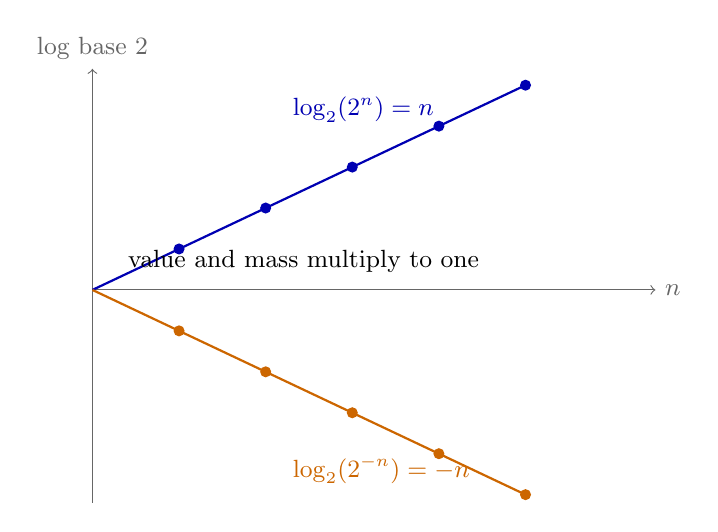
\begin{tikzpicture}[x=1.1cm,y=0.52cm]
\draw[->,black!60] (0,0)--(6.5,0) node[right,font=\small] {$n$};
\draw[->,black!60] (0,-5.2)--(0,5.4) node[above,font=\small] {log base 2};
\draw[blue!70!black,thick] (0,0)--(5,5);
\draw[orange!80!black,thick] (0,0)--(5,-5);
\foreach \n in {1,2,3,4,5}{\fill[blue!70!black] (\n,\n) circle[radius=2pt];\fill[orange!80!black] (\n,-\n) circle[radius=2pt];}
\node[blue!70!black,font=\small,anchor=west] at (2.2,4.4) {$\log_2(2^n)=n$};
\node[orange!80!black,font=\small,anchor=west] at (2.2,-4.4) {$\log_2(2^{-n})=-n$};
\node[font=\small,anchor=west] at (0.3,0.7) {value and mass multiply to one};
\end{tikzpicture}
